\chapter{Design}
\label{Design}
This chapter describes the proposed design of whole system for storing and exploring blockchains in IPFS that is to be
created as a result of this thesis. All parts of system are described in this chapter.

\section{Overview}
The system consists of one or more Feeders and Explorers. Feeders are connected to external API and provide synchronization between cryptocurrency and IPFS data. Explorer can request data from the system network and display them to user.

\begin{figure}[h]
    \centering
    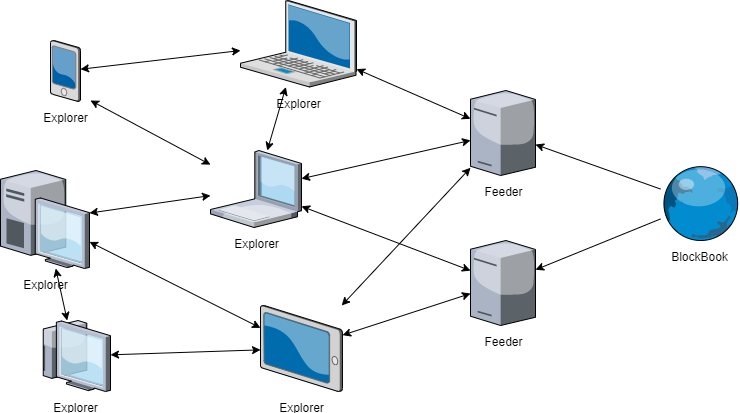
\includegraphics[width=11cm]{AppArchitecture.png}
    \caption{System design}
    \label{}
\end{figure}

\section{Blockbook}
Blockbook\footnote{\url{https://github.com/trezor/blockbook}} is a blockchain indexer for Trezor Wallet\footnote{\url{https://wallet.trezor.io/}}, developed by SatoshiLabs\footnote{\url{https://satoshilabs.com/}}. It currently supports more than 30 coins (and some others were implemented by the community). For data storage Blockbook is using RocksDB\footnote{\url{https://github.com/facebook/rocksdb/wiki}} developed by Facebook, which is a NoSql database which stores only key-value pairs. Blockbook is providing fast API for accessing blocks, addresses and transactions. Main limitations of blockbook:
\begin{itemize}
    \item \textbf{Not distributed} (client-server architecture) - problem with scalling for more users. 
    \item \textbf{Not a SQL database} - it does not have a relational data model, it does not support SQL queries, and it has no support for indexes.
    \item \textbf{Single-Process} - only a single process (possibly multi-threaded) can access a particular database at a time.
\end{itemize}

\section{Feeder}
A Feeder is a command-line service that stores data in IPFS for all cryptocurrencies specified in the config file. It uses Blockbook API for obtaining data. Feeder stores data in structure such as in figure \ref{feederDataStorageStructure}. Each block (except genesis and last block) has a link to the previous and next block. Also, it has links to transactions that had been processed in this block. A transaction has links to address and previous/spent transaction for every input/output. This scheme allows to store blockchain data in IPFS in small objects with size less than 256KB (a limit for storing objects directly in DHT). Also, every logical link between objects is preserved.


\begin{figure}[h]
    \centering
    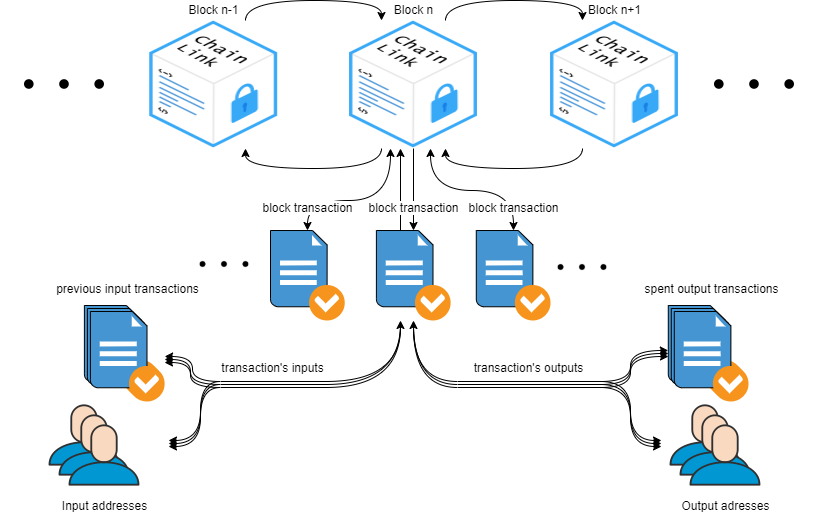
\includegraphics[width=12cm]{feederDataStorageStructure.png}
    \caption{Feeder data storage structure}
    \label{feederDataStorageStructure}
\end{figure}




\section{Explorer}
Explorer is an application providing simple GUI and API. Application is runnable in browser or Node.js\footnote{\url{https://nodejs.org/}}. Explorer can perform basic queries like a search for block by its height or hash and search address and transaction by hash. Nevertheless, depending on specified indexes in Feeder, Explorer can also make more complex queries, for example, get 20 transaction where the sum of inputs is more than 0.5, or get transactions between some time interval.



